%%%%%%%%%%%%%%%%%%%%%%%%%%%%%%%%%%%%%%%%%%%%%%%%%%%%%%%%%%%%%%%%%%%%%%%%%%%%%%%%%%%%%%%%%%%%%%%%%%%%%%
%
%   Filename    : chapter_2.tex 
%
%   Description : This file will contain your Review of Related Literature.
%                 
%%%%%%%%%%%%%%%%%%%%%%%%%%%%%%%%%%%%%%%%%%%%%%%%%%%%%%%%%%%%%%%%%%%%%%%%%%%%%%%%%%%%%%%%%%%%%%%%%%%%%%


\chapter{Review of Related Literature}
\label{sec:relatedlit}

This chapter discusses the features, capabilities, and limitations of existing research, as well as the algorithms and/or software that are relevant to the study. 

%section~~~~~~~~~~~~~~~~~~~~~~~~~~~~~~~~~~~~~~~~~~~~~~~~~~~~~~~~~~~~~~
\section{Data Extraction Tools}
Data extraction is the process of crawling through data sources, such as a database, in order to retrieve information that can be used for further data processing or data storage \cite{Technopedia2016}. For this study, data extraction involves selecting needed data from Facebook as an input to the story generation system. 

Three data extraction tools that are relevant to the current study have been reviewed:
\begin{enumerate}
\item Download Facebook Data \cite{FacebookDownload, FacebookDownload2}
\item Graph API \cite{WeaverTarjan2013, FacebookGraphAndroid2016}
\item Facepager \cite{Facepager2016}
\end{enumerate}

Table \ref{tab:DataExtractionTool} shows a comparison of these data extraction tools.

\subsection{Download Facebook Data}
The simple act of logging in to Facebook is already a way of accessing data stored in Facebook. The Activity Log is a built-in Facebook feature that shows the history of activities done on Facebook. It includes likes, comments, search history, and others. In 2010, Facebook introduced a new feature where these data can be downloaded for the user's own purposes. This is a compilation of the user's own data on Facebook, such as the user's personal info, friends list, and messages, among others.

Facebook automatically compiles the data to be downloaded once the user chooses to archive his/her files. An email containing the download link would then be forwarded to the mail address registered in the user's account. Once downloaded, the .zip file includes all media posted by the user in Facebook. It also contains a file, index.html, which is an HTML file that acts similarly to Facebook's home page. It displays the user's profile data such as the Facebook link, email address, registration date, birthday, past Facebook names (if any), current city and hometown, and other information that the user has provided on this Facebook account. There are also several HTML files provided in the HTML folder for easier indexing and browsing, as shown in \figref{fig:fbdatazip}.

\begin{figure}[!htb]                %-- use [t] to place figure at top, [b] to place at the bottom, [h] for here
   \centering                    %-- use this to center the figure
   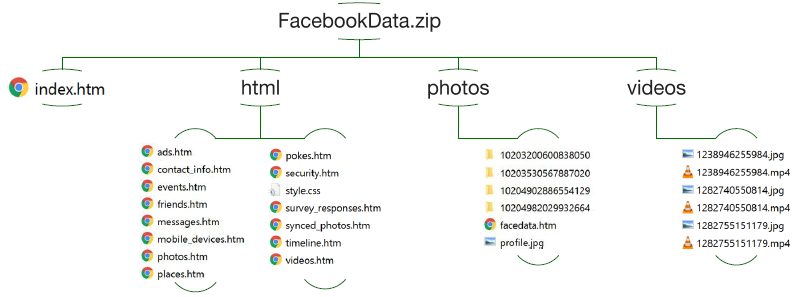
\includegraphics [width=\textwidth] {fbdatazip.png}      %-- include image file named as "disneychart.png" 
   \caption{Content of Facebook Data .zip File}
    \label{fig:fbdatazip}
\end{figure}

The date, time, timezone, tags, and source of posts that are shared are provided in the Timeline tab. Meanwhile, image and video files are separated from the description that comes along with it. Similar to the Timeline tab, the photos and videos tab also contains the time, date, and timezone of the media file posted. Aside from displaying the media file and the missing message of the post, the photos include the following details - the camera model, orientation, width, exposure, ISO speed, IP address and comments - while the videos include the thumbnail image and comments in the video.

\subsection{Graph API}
Facebook has developed the Graph API to allow developers to extract posts and other data from a specific Facebook page or a user's Facebook account. The API can be accessed from the URL, developer.facebook.com/tools, once a user has logged in.

Facebook's Graph API supports developers by supplying services such as providing snippets of codes for easier integration in JSON requests and responses. In \figref{fig:graphplatforms}, GraphRequest calls ``/user/me" to fetch the user data for the given access token. An access token controls data access and contains the permissions that the user has allowed, as seen in \figref{fig:graphpermissions}. This access token expires after one hour. If no access token is provided, Graph API would only return publicly available information. The response data is deserialized into a JSONObject if the request is successful.

\begin{figure}[!htb]                %-- use [t] to place figure at top, [b] to place at the bottom, [h] for here
   \centering                    %-- use this to center the figure
   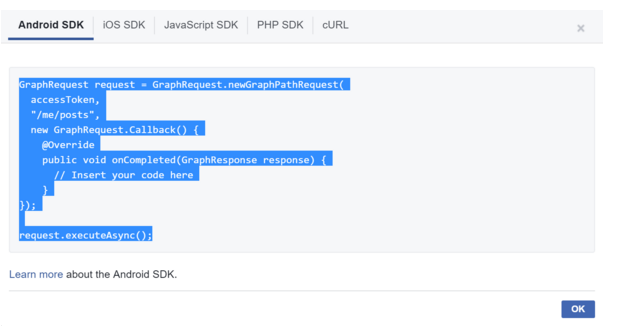
\includegraphics [width=5in,height=3in,keepaspectratio] {graphplatforms.png}      %-- include image file named as "disneychart.png" 
   \caption{Available Coding Platforms and Code Snippets in Graph API} \cite{FacebookGraphAndroid2016}
    \label{fig:graphplatforms}
\end{figure}

\begin{figure}[!htb]               %-- use [t] to place figure at top, [b] to place at the bottom, [h] for here
   \centering                    %-- use this to center the figure
   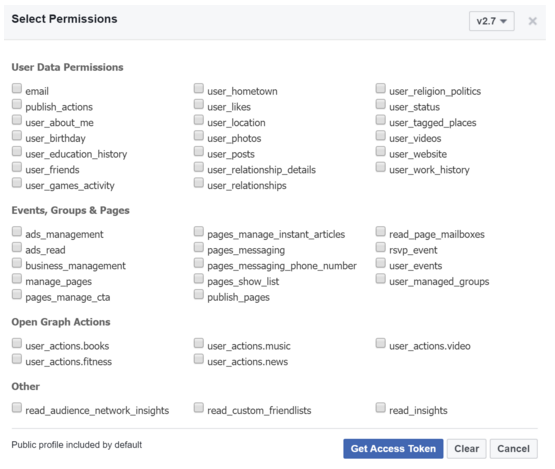
\includegraphics [width=5in,height=4in,keepaspectratio] {graphpermissions.png}      %-- include image file named as "disneychart.png" 
   \caption{Permissions in an Access Token} \cite{FacebookGraphAndroid2016}
    \label{fig:graphpermissions}
\end{figure}

\clearpage
\subsection{Facepager}
Facepager is a free and open-source tool that has gained quite a lot of interest for its simple process of collecting data through application program interfaces (APIs). Using Facepager does not require knowledge of programming because of its simple design. Presets are also available to help beginners and first time users when working with Facepager. Students and researchers commonly use this tool to gather data for projects such as for analyzing political communication on Facebook, and market analysts also make use of this tool to analyze data regarding a certain product.

Public data from Facebook, such as pages of companies or artists, enables Facepager to extract the content of the post, the number of likes, shares, and comments as well as other details provided. 

Data are collected and extracted depending on the provided object ID or Facebook page name. All these collected data are then stored in a SQLite database that could later be exported to a Comma Separated Values (CSV) file for further analysis. Each row or tuple would contain the name of the page, message, type (indicated whether it is a video, link, photo), metadata type, likes, likes count, shares count, comments count, time it was created as well as the time the post was updated.

\clearpage
\begin{sidewaystable}[ph!]   %t means place on top, replace with b if you want to place at the bottom
\centering
\caption{Comparison among the different data extraction tools.} \vspace{0.25em}
\begin{tabular}{|p{1in}|p{4cm}|p{3cm}|p{3cm}|p{3cm}|p{2cm}|p{1cm}|p{2cm}|} \hline
\centering Data Extarction Tool & Data being extracted & Extraction of Data & Input & Output & Domain & Free & Platform \\ \hline
Download Facebook Data  & Activity Log; \newline User Profile Information; \newline Messages; \newline Friend List & Facebook User Account & N/A \newline *Only requires user to log in*  &  Zip file containing html files and the media files &  Facebook & Yes & HTML\\ \hline
Graph API & Activity Log; \newline User Profile Information  & Facebook Pages or Facebook User Account & Object ID and Access Token & JSON Object & Facebook & Yes & JavaScript \newline PHP \newline Android SDK \newline iOS SDK \newline cURL \\ \hline
Facepager & Facebook resources
 & Public Facebook Pages; \newline Public Twitter pages; \newline Public youtube accounts & Object ID & Data stored in SQLLite or CSV & Facebook \newline Twitter \newline Youtube & Yes & Python\\ \hline
\end{tabular}
\label{tab:DataExtractionTool}
\end{sidewaystable}
\clearpage

%section~~~~~~~~~~~~~~~~~~~~~~~~~~~~~~~~~~~~~~~~~~~~~~~~~~~~~~~~~~~~~~
\section{Text Understanding Tools}
Text understanding is the process of inferring the intended meanings of text made in natural language, such as greetings, commands, or messages. It consists of (1) reading texts that were formed in natural language; (2) determining the implicit and explicit meaning of each element, including words, phrases, sentences, and paragraphs; and (3) making inferences based on the implicit and explicit properties of these texts \cite{ZhangLecun2015}.

Text understanding tools are relevant in this research as a means of interpreting the textual contents extracted from Facebook. The text understanding tools reviewed in this study are the following:
\begin{enumerate}
\item FastText \cite{FastText2016, Techcrunch2016}
\item DeepText \cite{DeepText2016}
\item Google Cloud Natural Language API \cite{GoogleAPI2016}
\item Stanford CoreNLP \cite{Manning14thestanford}
\end{enumerate}

Table \ref{tab:TextUnderstandingTool} shows a comparison of these text understanding tools.

\subsection{FastText}
FastText is an open-source library for building text representation and classification \cite{FastText2016}. It combines a number of language processing and machine learning concepts introduced in recent years, such as bag of n-grams and subword information. Different concepts are employed for two main purposes: efficient text classification, and learning word vector representations.

The bag of n-grams process is fast because it focuses more on the occurrences of a word as opposed to word order \cite{Techcrunch2016}. Words are represented in a multidimensional space, and linear algebra is used to calculate the relationship between a query and a categorized set of words. Via this method, a problem which is \textit{qualitative} in nature-- text analysis-- becomes qualitative through the addition of statistics. Essentially, this enables fastText to be faster than traditional deep learning methods. \figref{fig:FastText} shows a comparison between fastText and other text representation libraries. 

\begin{figure}[!htb]               %-- use [t] to place figure at top, [b] to place at the bottom, [h] for here
   \centering                    %-- use this to center the figure
   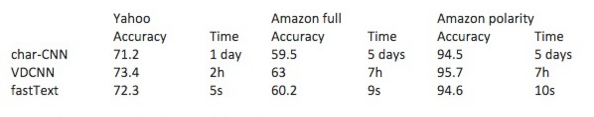
\includegraphics {FastText.png}      %-- include image file named as "disneychart.png" 
   \caption{A comparison between fastText and deep learning-based methods.}
    \label{fig:FastText}
\end{figure}

FastText is not restricted to English and can work with other languages including German, Spanish, French, and Czech \cite{Techcrunch2016}.

\subsection{DeepText}
DeepText is a ``deep learning-based text understanding engine." It can understand with near-human accuracy the textual content of several thousand posts per second \cite{DeepText2016}. It aims to help users make tasks, such as defining words or reserving plane tickets, easier.

Facebook users are composed of people with different cultures. Thus, it is important for DeepText to be able to interpret as many languages as possible. Another goal of DeepText is to better understand words in different languages using labeled data instead of traditional NLP techniques that would normally take longer processing time. In traditional NLP, the understanding part is highly dependent on stored knowledge thus requiring each word to be exactly the same for it to be understood. However, with deep learning, word embeddings could be used to get a sense of the word. According to Facebook, it is a ``mathematical concept that preserves the semantic relationship among words". By mapping words and phrases into a common embedding space, it might know which words written in different languages yield the same meaning.

\subsection{Google Cloud Natural Language API}
The Google Cloud Natural Language API offers powerful text analysis by using machine learning models that are capable of revealing the structure and meaning of text. It can extract information about entities (such as people or places) which can be found in documents, articles, or blogs. Google uses the same machine learning technology to understand and answer user questions in a Google search query.

The Natural Language API features syntax analysis, entity recognition, multi-language, and integrated REST API. Syntax analysis is the process of extracting tokens and sentences, identifying the different parts of speech, and creating dependency parse trees for each sentence. Entity recognition seeks to locate and classify entities in text into predefined categories such as person, organization, location, events, and media. The API allows analysis of text in different languages, including English, Japanese, and Spanish. And lastly, the integrated REST API allows text to be uploaded in the request or integrated with Google Cloud Storage.

The API has several methods for performing analysis on text and each level of analysis provides valuable information for text understanding. One method is [1] syntactic analysis, which consists of the following operations: (1) sentence extraction, (2) tokenization, and (3) mapping. These will help in determining the syntactic meaning of tokens and their relationships. Syntactic analysis, as shown in \figref{fig:google-syntax}, is used for analyzing and parsing text.

\begin{figure}[!htb]                %-- use [t] to place figure at top, [b] to place at the bottom, [h] for here
   \centering                    %-- use this to center the figure
   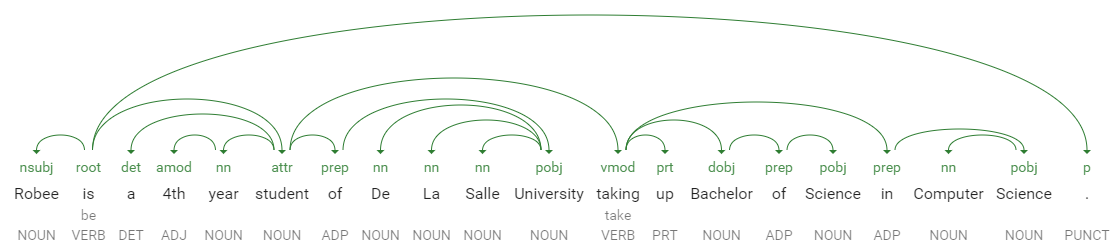
\includegraphics [width=\textwidth] {google-syntax.png}      %-- include image file named as "disneychart.png" 
   \caption{Sample output for syntax analysis}
    \label{fig:google-syntax}
\end{figure}

Another method is [2] entity analysis, as shown in \figref{fig:google-entities}. It is useful for disambiguating similar entities and providing information about each entity found in the text. The analysis returns a set of detected entities, and parameters that are in connection with the identified entities, such as the type of the entity, its relevance to the text, and positions within the text where the identity was mentioned. Each entity is ordered from highest to lowest according to their salience scores, which reflects their importance in the overall text. Scores closer to 1.0 are highly salient, while scores closer to 0.0 are less salient. 

\begin{figure}[!htb]                %-- use [t] to place figure at top, [b] to place at the bottom, [h] for here
   \centering                    %-- use this to center the figure
   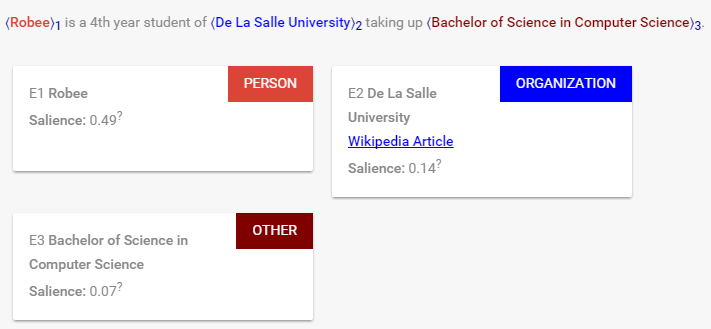
\includegraphics [width=\textwidth] {google-entities.png}      %-- include image file named as "disneychart.png" 
   \caption{Sample output for entity recognition}
    \label{fig:google-entities}
\end{figure}

\subsection{Stanford CoreNLP}
Stanford CoreNLP is a Java-based annotation pipeline framework which provides a set of natural language technology analysis tools ranging from tokenization to coreference resolution \cite{Manning14thestanford}. It supports text in different languages such as Arabic, Chinese, English, French, German, and Spanish.

Stanford CoreNLP has several options to choose from when doing syntax analysis. But before the actual syntax analysis, it must first perform two operations: (1) sentence extraction and (2) tokenization. Sentence extraction is the process of breaking down the text into separate sentences, while tokenization is the act of breaking down a sentence into tokens.

After that, the choices for syntax analysis include: (a) part-of-speech tagging (shown in \figref{fig:new-postag}), (b) named entity recognition (shown in \figref{fig:new-ner}), (c) lexical parsing (shown in \figref{fig:new-parsetree}), or (d) universal dependencies (shown in \figref{fig:new-dependencies}). Part-of-speech tagging returns the part of speech of each token; named entity recognition returns proper nouns; lexical parsing analyzes the grammatical structure of each sentence and provides a dependency tree; and the universal dependencies shows the relationship of a word to other words.

\begin{figure}[!htb]                %-- use [t] to place figure at top, [b] to place at the bottom, [h] for here
	\centering                    %-- use this to center the figure
	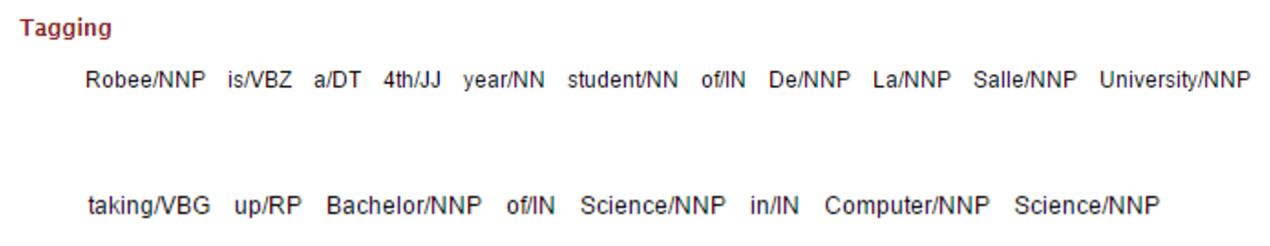
\includegraphics [width=\textwidth] {new-postag.png}      %-- include image file named as "disneychart.png" 
	\caption{Sample Part-of-speech Tagging using Stanford CoreNLP} 
	\label{fig:new-postag}
\end{figure}

\begin{figure}[!htb]                %-- use [t] to place figure at top, [b] to place at the bottom, [h] for here
	\centering                    %-- use this to center the figure
	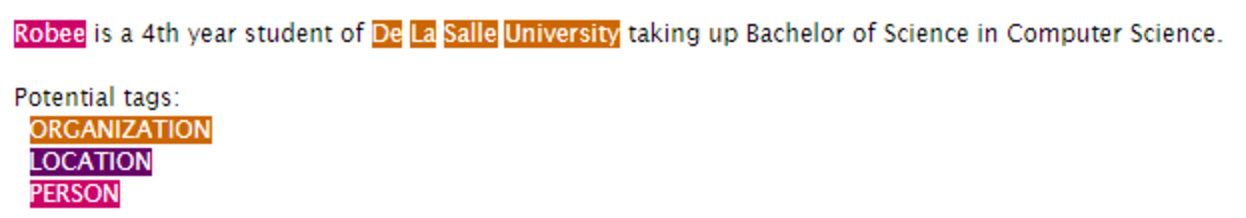
\includegraphics [width=\textwidth] {new-ner.png}      %-- include image file named as "disneychart.png" 
	\caption{Sample Named Entity Recognition using Stanford CoreNLP} 
	\label{fig:new-ner}
\end{figure}

\begin{figure}[!htb]                %-- use [t] to place figure at top, [b] to place at the bottom, [h] for here
	\centering                    %-- use this to center the figure
	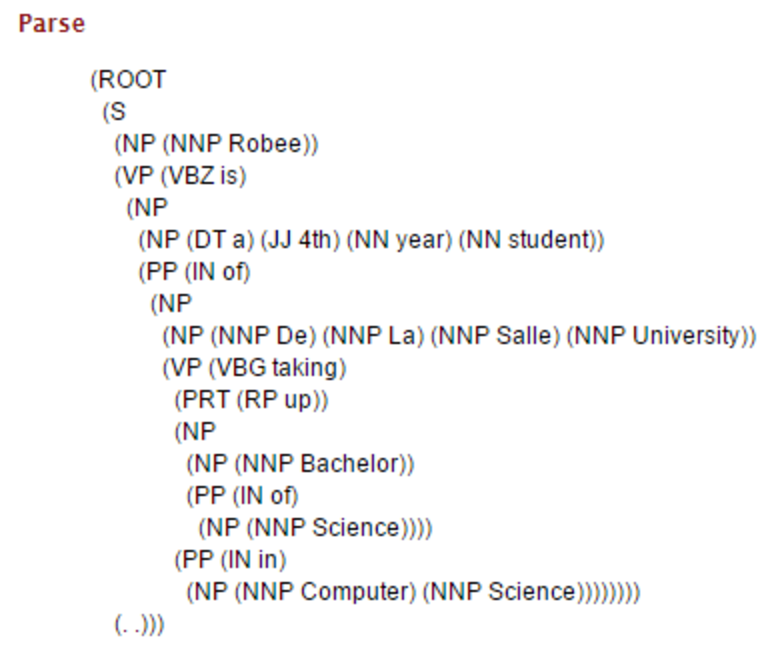
\includegraphics{new-parsetree.png}      %-- include image file named as "disneychart.png" 
	\caption{Parse Tree Output by Stanford CoreNLP} 
	\label{fig:new-parsetree}
\end{figure}

\begin{figure}[!htb]                %-- use [t] to place figure at top, [b] to place at the bottom, [h] for here
	\centering                    %-- use this to center the figure
	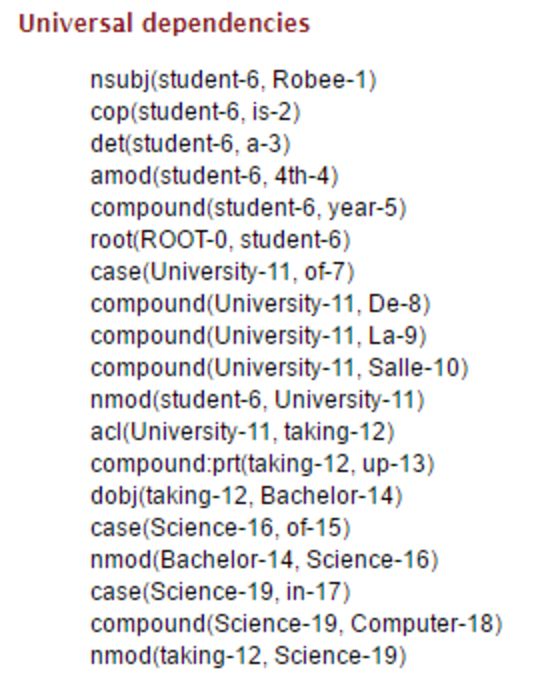
\includegraphics{new-dependencies.png}      %-- include image file named as "disneychart.png" 
	\caption{Universal Dependencies Output by Stanford CoreNLP} 
	\label{fig:new-dependencies}
\end{figure}

\clearpage
\begin{table}[ph!]   %t means place on top, replace with b if you want to place at the bottom
\centering
\caption{Comparison of the text understanding tools.} \vspace{0.25em}
\begin{tabular}{|p{1in}|p{1.5in}|p{1.5in}|p{1in}|} \hline
\centering Text Understanding Tool & Learning Process & Processes Available & Languages Supported \\ \hline
FastText & You have to train it yourself & Classification of posts & English, German, Spanish, French, and Czech \\ \hline
DeepText & Used FBLearner Flow and Torch for model training. & Entity recognition, General classification about the posts, extracting intent, and sentiment analysis & More than 20 languages \\ \hline
Google Cloud Natural Language API & Pre-trained & Entity recognition, Sentiment analysis, and Syntax analysis & English, Spanish, and Japanese \\ \hline
Stanford CoreNLP & Pre-trained & Arabic, Chinese, English, French, German, and Spanish & Part-of-Speech Tagger, Named Entity Recognition, Parser, Sentiment Analysis, Coreference, Universal Dependencies, Lemmatizer \\ \hline
\end{tabular}
\label{tab:TextUnderstandingTool}
\end{table}

%section~~~~~~~~~~~~~~~~~~~~~~~~~~~~~~~~~~~~~~~~~~~~~~~~~~~~~~~~~~~~~~
\section{Story Generation Systems}
Story generation systems output a complete story of a certain genre given a (usually) unique set of inputs. The following story generation systems are reviewed in three aspects - the different inputs accepted and the output generated; and the process of planning the story:
\begin{enumerate}
\item Novel Writer System \cite{Gervas2012, Gervas2009, MendezGervasDeleon2014, LaclaustraLedesmaMendezGervas2014}
\item TALE-SPIN \cite{Gervas2009, Mawhorter2013, Meehan1977}
\item Picture Books \cite{SolisSiyTabiraoOng2009, angenhancing, picbooks4}
\item Learning To Tell Tales \cite{McIntyreLapata2009}
\end{enumerate}

Table \ref{tab:StorytellingSystems} shows a comparison among these story generation systems.

\subsection{Novel Writer System (1973)}
The first ever storytelling system was the Novel Writer System developed by Sheldon Klein. The system was recorded to have generated 2100-word murder-mystery stories in less than 19 seconds \cite{Gervas2012}. It uses a microsimulation model in which the behavior of each character and events were ruled by probabilistic rules that continuously changes the story \cite{Gervas2009}.

The user has to provide the character traits of the murderer/s and the victim/s with additional traits that describe their relationships with each other, their tendency to commit violence or sex, and the description of the setting in which the story will take place \cite{Gervas2012,  MendezGervasDeleon2014, LaclaustraLedesmaMendezGervas2014}. During the course of the story, some of the events causes motives to arise. Greed, anger, jealousy, and fear are possible motives for murder. The system can also generate more than one text-based story, indicating who the murderer is, why the murder was committed, and who discovered the murder incident.

The system generates stories based on two different algorithms: (1) a set of rules that indicates the possible changes from the current state of the story to the next and (2) a sequence of scenes corresponding to the type of story to be told. There are pre-defined set of rules to allow the construction of only one specific type of story.

\subsection{TALE-SPIN (1977)}
TALE-SPIN is a storytelling system that generates stories about the lives of  woodland creatures developed by James Meehan \cite{Gervas2009}. It uses character simulation as a method in creating stories \cite{Mawhorter2013}.

The user chooses the traits and morals of the characters as well as the problem they will be facing \cite{Gervas2009, Meehan1977}. As the story progresses, new characters and items will be added as needed \cite{Meehan1977}. Relationships between the character may also arise to competition, dominance, familiarity, among others \cite{Gervas2009}. The system then generates a story containing the events that are to happen in order to solve the problem.

The story has three main components: (1) the problem solver, (2) the goal, and (3) the sub-goals and actual events \cite{Meehan1977}. TALE-SPIN generates stories by combining both backward and forward chaining \cite{Meehan1977}. Forward chaining is expounding on the available data to be able to extract more data until the end goal is obtained, while backward chaining is described as working backward from the given goal/s, tracking down events that will yield the solution to the problem.

\subsection{Picture Books (2008-2015)}
Picture Books 1-4 is a series of existing automated story generation systems which use picture elements (setting, characters and items) as inputs from children in producing a fable-like text-based story. Stories are generated using Natural Language Generation (NLG) techniques. The stories to be generated follow the plot structure of exposition, rising action, climax and resolution.

The architectural design of Picture Books 1 is composed of three modules: the picture editor, the story planner and the sentence generator. The picture editor starts after the user chooses the setting of the story and the selection of characters and items come right after choosing the setting. The story planner module is subdivided into two modules: the story content planner and the story organizer. The story content planner chooses a theme based on the setting and items. The story organizer arranges and organizes the events of the story in an organized manner for the user. The result of this will be a story tree that will be used in the next module.  The sentence generator module is again subdivided into two modules: the sentence planner and realizer. The sentence planner converts the story tree from the story organizer to sentence templates. The realizer then uses the SimpleNLG realiser which is an open source Java class library in converting the sentence templates given by the sentence planner to the actual sentences that made up the story. The final output of the realizer includes the story title and the story itself.

Picture Books 2 targets a slightly older age group comprising of children aged six to eight years old \cite{ang2010generating}. It creates a more creative environment through depicting stories in a sequence of scenes through the given images and characters provided. The new environment required new semantic relations to be added to define the concepts dealing with movements and positioning of the objects in the story. It is capable of developing three or more scenes portraying various scenes in the intended story where in the characters exhibit three traits assigned by the system which helps depicts the story to the children. The system structure is similar to Picture Books 1 starting with the story editor module which initializes the environment for the user. The story planner module experienced changes as it aims to impart a moral lesson to the user with the use of the character's actions. It is comprised of three modules, mainly the theme formulator, setting formulator, and event generator. The theme formulator identifies the background, character and objects present in the scene and formulates a theme defining the character trait that it lacks for further development. The setting formulator focuses on describing the location and time the story takes place which is identified through a grid placed in the scene. Events generation involves the conceptual relations on the specified theme. Lastly, the sentence planner transforms the sequence of conceptual relations using character goals into readable sentences which involves aggregation, lexicalization and referencing.

In Picture Books 4, the system automatically generates stories based on pictures or stickers the children puts on the scene \cite{picbooks4}. Similar to Picture Books 2, it focuses on children from six to eight years old. It has the capability of generating stories consisting of single to multiple scenes, and can generate stories with a single character or with multiple characters, however, it focuses more on developing stories with multiple characters by incorporating interaction between them. Unlike Picture Books 1 and 2, which only caters one type of interaction, character-to-object, and character-to-character interaction, respectively, Picture Books 4 caters to both types of interaction and two additional types of interaction which are the verbal interaction and non-verbal interaction. The system uses both character-centric and author-centric approaches. The character-centric approach allows characters to have their own individual goals and pursue these goals in a way that is consistent with their personality and desires, while the author-centric approach makes sure that the entirety of the story revolves around the main topic. The system has three modules that were adapted from previous Picture Book systems. 

\subsection{Learning To Tell Tales (2009)}
Learning To Tell Tales is a data-driven approach in storytelling \cite{McIntyreLapata2009}. The user provides the topic that may come in the form of phrase or sentence and the desired length of the story. The output is a text-based story generated after looking in the knowledge base containing the topic.

The system conceptualizes the story generation process as a tree after consulting the knowledge base. The story tree \figref{fig:storytree} has different levels which represent the number of sentences to be generated in the output. Additionally, each sentence in the tree has their own score. To generate a story, the system traverses the tree and chooses the node with the highest score. The system also uses two different searching methods: (1) searching for the best story and (2) searching for the most suitable sentences that can be gathered from the knowledge base.

\begin{figure}[!htb]                %-- use [t] to place figure at top, [b] to place at the bottom, [h] for here
   \centering                    %-- use this to center the figure
   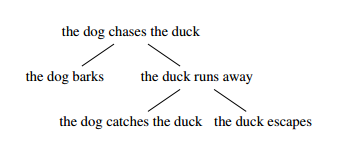
\includegraphics{storytree.png}      %-- include image file named as "disneychart.png" 
   \caption{Example Story Tree} \cite{McIntyreLapata2009}
    \label{fig:storytree}
\end{figure}

There are four modules in order to generate a story: (1) content planning, (2) sentence planning, (3) surface realization, and (4) story ranking. First, all the possible verb-subject, verb-object, verb-adverb, and noun-adjective relations related to the topics are extracted from the corpora stored in the knowledge base and each of these verbs will have a score. Second, the system must combine each of them to form a sentence. The grammar rules will act as a template. Third, the sentences will undergo surface realization which fixes the grammar of each sentence. Lastly, the system performs a story ranking to know whether the story generated is interesting and coherent.

\clearpage

\begin{sidewaystable}[ph!]   %t means place on top, replace with b if you want to place at the bottom
\centering
\caption{Comparison among the different story generation systems.} \vspace{0.25em}
\begin{tabular}{|p{1in}|p{2cm}|p{2cm}|p{2cm}|p{2cm}|p{2cm}|p{2cm}|p{2cm}|p{2cm}|} \hline
\centering Story Generation System & Genre & Target & Theme & Input & Output & Approach & Goal \\ \hline
Novel Writer System & Murder & Not specified & Weekend party & Murderer/s \newline Victim/s \newline Description of Setting & Text-based story & Rule-based & No\\ \hline
TALE-SPIN & Aesop's Fable-like stories & Not specified & Not specified & Initial Setting \newline Traits or morals of characters \newline Goal & Text-based story & Not Specified & Yes \\ \hline
Picture Books & Fable & Children (age 4 to 6) & Not specified & Settings \newline Character \newline Items & Text-based story & Author-centric \newline Character-centric & No \\ \hline
Learning To Tell Tales & Not specified  & Young Children  & Depends on the gathered information & Topic \newline Length of Story & Text-based story (based on the length specified by the user) & Knowledge-based reasoning & No \\ \hline
\end{tabular}
\label{tab:StorytellingSystems}
\end{sidewaystable}
\clearpage

%section~~~~~~~~~~~~~~~~~~~~~~~~~~~~~~~~~~~~~~~~~~~~~~~~~~~~~~~~~~~~~~
\section{Social Networking Sites}
Social networking sites (SNS) are popular tools for social interaction as well as information exchange between individuals \cite{HughesRoweBateyLee2012}. They serve as virtual communities which allow people to connect and interact with each other on a  particular subject, or to just ``hang out'' together online \cite{CheungChiuLee2011}.

The social networking sites reviewed here are Facebook and Twitter.

\subsection{Twitter}
Twitter is commonly referred as a micro-blogging website. This is a combination of instant messaging and blogging that allows users to post or send a short message, but is limited to 140 characters, called ``tweets'' \cite{Crymble2010}. In 2010, Twitter's population grew to 175 million registered users from 30 million users early that year \cite{Rao2010}. Registered users can read and post tweets, retweet other's tweet, and follow other users or industry figures for updates, while unregistered users can only read tweets from public accounts.

Twitter has become popular in today's society for several reasons. It is one of the first sites to introduce the \textit{following} and \textit{followers} concepts that appeal to the audience as they can easily follow or unfollow other users. It is also one of the most simple social media sites to use because of its simplicity and easily navigable interface. In addition, Twitter allows users to easily share information.

However, Twitter has some downsides. First, there is no system of accuracy as users can just say about anything. Second, users are limited to 140 characters, which means, they may not be able to explain themselves or their thoughts in detail. Many tweets involve either a use of  ``(con't.)'' and/or a reply to the own tweet to signify a chain of tweets that are altogether expressing a single thought. And lastly, Pear Analytics, a firm that specializes in marketing analytics, conducted a study that categorized tweets into 6 areas - News, Spam, Self-Promotion, Pointless Babble, Conversational and Pass-Along Value. They found out that 40.55\% of the tweets in the gathered sample fit into the category of Pointless Babble, followed by a 37.55\% in conversational \cite{PearAnalytics2009}.

\subsection{Facebook}
Facebook is the most active SNS today. It consists of multiple avenues of social interactions and billions of page views, with more than 21 million users as of 2007 \cite{EllisonSteinfieldLampe2007} and has dramatically increased to almost one billion users worldwide as of 2013 \cite{FarahbakhshHanCuevasCrespi2013}. The comScore Media Metrix Multi-Platform conducted a study in 2015 showing a huge gap between other social networks and Facebook for being the most accessed site for millennials as shown in \figref{fig:snsdemographics} below. According to Dave Chaffey \citeyear{Chaffey2016}, Facebook continues to dominate the social landscape, leading number one on social media platforms around the world.

\begin{figure}[!htb]                %-- use [t] to place figure at top, [b] to place at the bottom, [h] for here
	\centering                    %-- use this to center the figure
	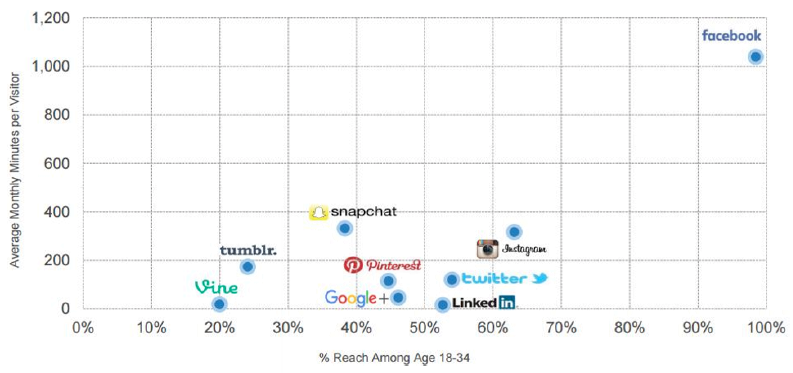
\includegraphics [width=\textwidth]{snsdemographics.png}      %-- include image file named as "disneychart.png" 
	\caption{Millennial Demographics in Social Media Platforms } \cite{Chaffey2016}
	\label{fig:snsdemographics}
\end{figure}

Facebook is a convenient and open social media platform that welcomes not just individuals but also companies and organizations to communicate and interact with one another. Westlake \citeyear{Westlake2008} states that ``Facebook develops technologies that facilitate the spread of information through social networks allowing people to share information online the same way they do it in the real world''. It promotes interactions between users, through simple status updates, posts, or shares, and enables users to inform others about their whereabouts and actions.

In Facebook, users are required to create visible profiles providing their name, gender, date of birth and email address. In addition to that, more information such as contact information, personal interests, background information and favorites (books, movies and music) can also be added to the profile at the discretion of the user \cite{NadkarniHofmann2012}. Posting information about their interest enables others to get a grasp of one's characteristics or personality \cite{FarahbakhshHanCuevasCrespi2013}. Derek Coles \citeyear{Doughty2015} said that ``Facebook is the modern way of not being on your own'' as it also allows you to interact and meet people you don't know and enables people to discuss topics with common interests. 

A study by Ashwini Nadkami and Stefan G. Hofmann \citeyear{NadkarniHofmann2012}, showed that people tend to stay online and use Facebook because posting in Facebook allows self-promotion and influences one's self-esteem and self-worth. Self-esteem and self-worth are affiliated with the sense of belonging in the society or a acceptability to a group, which, according to Nadkami \& Hoffman, can be measured by the number of likes and comments received on one's share or post or a simple act like being tagged in a group picture. The study concluded that ``Facebook creates an environment where information is shared proactively because of the site's influence on a  user's need for popularity'' \cite{NadkarniHofmann2012}.

%section~~~~~~~~~~~~~~~~~~~~~~~~~~~~~~~~~~~~~~~~~~~~~~~~~~~~~~~~~~~~~~
\section{Knowledge Base}
According to the American Heritage Dictionary (2011), a \textit{knowledge} base is a collection of data organized in a form that facilitates analysis by automated deductive processes. It can be perceived as an expert system \cite{mars1995towards}. It uses a \textit{knowledge representation language} for expressing rules and/or objects.

The different knowledge base systems reviewed in this section are as follows:
\begin{itemize}
\item Cyc \footnote{OpenCyc. http://www.opencyc.org/} \cite{cyc1999, cycinferencing1994};
\item WordNet \footnote{WordNet. https://wordnet.princeton.edu/}; and
\item ConceptNet \cite{LiuSingh2004}.
\end{itemize}

Table \ref{tab:KnowledgeBase} shows a comparison among these knowledge base systems.

\subsection{Cyc}
Cyc is an artificial intelligence project that aims to collate and assemble a complete knowledge base of everyday common sense knowledge that humans inherently have \footnote{Cyc. http://psych.utoronto.ca/users/reingold/courses/ai/cyc.html}. This project is undertaken with the goal of enabling applications that use AI to perform reasoning that can be considered humanlike.

Cyc's knowledge base consists of data from news and magazine articles, encyclopedia entries, advertisements, and more. Cyc's knowledge base is represented as a directed graph containing the following:
\begin{enumerate}
	\item Constants - terms that people understand;
	\item Variables - case-sensitive unique identifiers;
	\item Predicates - terms to represent relation types;
	\item Formulas - expressions;
	\item Logical connectors - and, or, not, implies;
	\item Quantifiers - forAll, thereExists;
\end{enumerate}

\figref{fig:cyc} shows an excerpt of Cyc's knowledge base. Fido (variable) is a (predicate) dog (constant), for example.

\begin{figure}[!htb]                %-- use [t] to place figure at top, [b] to place at the bottom, [h] for here
	\centering                    %-- use this to center the figure
	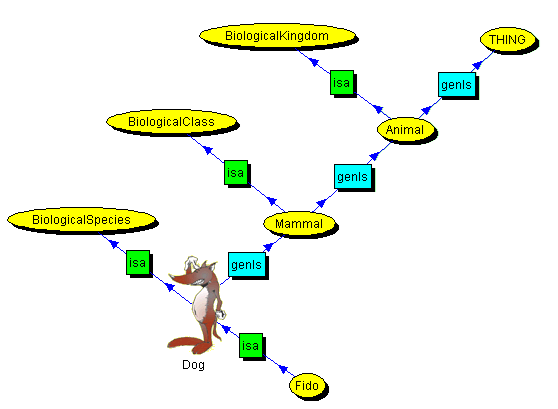
\includegraphics {cyc.png}      %-- include image file named as "disneychart.png" 
	\caption{An excerpt of Cyc's knowledge base, showing common sense knowledge about a dog named Fido.}
	\label{fig:cyc}
\end{figure}

Parts of the project were released to the public as OpenCyc, which provides an API, RDF redpoint, and data dump, all open-source \footnote{OpenCyc. http://www.opencyc.org/}. As of OpenCyc 2.0, the knowledge base contains 239,000 concepts and 2,093,000 facts, and can be browsed on the OpenCyc website. The CycL and SubL interpreter (the program that allows you to browse and edit the database as well as to draw inferences) is released free of charge, but only as a binary, without source code. It is available for Linux and Microsoft Windows.

Cyc also contains an inference engine -- that is, a computer program that derives answers from a knowledge base \footnote{Cycorop. http://www.cyc.com/overview-cyc-inferencing/}. The Cyc inference performs general logical deduction, used for reasoning.

\subsection{WordNet}
WordNet  \footnote{WordNet. https://wordnet.princeton.edu/} is a large lexical database of English words. A lexical database is a database of words and information about those words; in other words, a lexical database is a dictionary that is easily machine-readable according to The Free Dictionary \footnote{The Free Dictionary. http://www.thefreedictionary.com/}. In particular, WordNet is a database of words, primarily nouns, verbs, and adjectives, grouped into synonym sets, or ``synsets''. Rather than simply words, however, WordNet contains specific ``senses'' of words (a ``sense'' is a distinct meaning that a word can assume). These senses are linked to each other by semantic relations such as synonymy and ``is-a'' hierarchical relations (e.g. ``dog is a mammal'').

As of WordNet 2.0, the database contains around 200,000 word senses \cite{LiuSingh2004}. It is praised for being easy to use. As a simple semantic network with words at the nodes, it can be readily applied to textual input for purposes of getting more relevant results from a simple query, or determining semantic similarity between words.

\subsection{ConceptNet}
ConceptNet is a free common sense knowledge base and NLP toolkit developed by Hugo Liu and Push Singh \citeyear{LiuSingh2004}. Its information is based from the Open Mind Common Sense (OMCS) database. OMCS is an artificial intelligence project based on the Massachusetts Institute of Technology (MIT) Media Lab, and its goal is to create and maintain a large common sense knowledge base from the contributions of many people. In comparison to Cyc and WordNet, therefore, ConceptNet's knowledge base was filled in most part by the general public, rather than hiring a lot of knowledge engineers.

Common sense knowledge is knowledge that is inherent in most humans, enabling us to, for example, determine that a lemon is sour, a doorknob needs to be turned in order to open a door, or even why the sentence, ``I got fired from my job today,'' contains a negative connotation. 

ConceptNet's semantic network is expressed as a directed graph whose nodes are concepts which have atomic meaning (such as words like ``chair'', or phrases such as ``wake up''). These nodes are connected to each other by common sense knowledge about them. For example, ``waking up in the morning'' includes ``yawning'' and ``checking messages'' as its subevents as shown in \figref{fig:conceptnet}

\begin{figure}[!htb]                %-- use [t] to place figure at top, [b] to place at the bottom, [h] for here
	\centering                    %-- use this to center the figure
	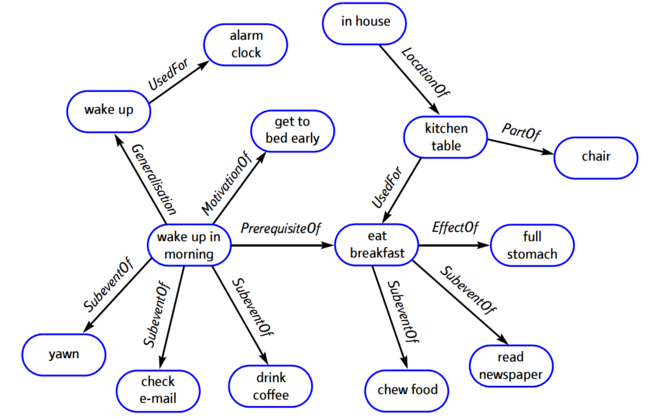
\includegraphics [width=4.5in,height=3.5in,keepaspectratio] {conceptnet.png}      %-- include image file named as "disneychart.png" 
	\caption{An example of ConceptNet's semantic network of knowledge. Concepts consist of a noun phrase along with an optional verb or prepositional phrase.}
	\label{fig:conceptnet}
\end{figure}

As of ConceptNet 5.0, there are over 3.9 million concepts, connected by 8.7 million assertions, such as ``IsA'' (``dolphin is a mammal''), ``LocationOf'' (``house is the location of kitchen table''), or ``SubeventOf'' (``chewing food is a subevent of eating breakfast'').

Through ConceptNet, it is easier to extract practical knowledge from text. This includes distinguishing between the correct definition of the word used in a context (``He ate chips with his lunch''), determining analogies, summarizing a topic, and event prediction.

\clearpage
\begin{sidewaystable}[ph!]   %t means place on top, replace with b if you want to place at the bottom
	\centering
	\caption{Comparison among the different knowledge base systems.} \vspace{0.25em}
	\begin{tabular}{|p{1.5in}|p{1.5in}|p{1.5in}|p{1.5in}|p{1.5in}|} \hline
		\centering Knowledge Base & Knowledge Objects & Relations & Content & Source of Knowledge \\ \hline
		Cyc & words & any & common sense data & magazine, news articles, encyclopedia, etc. \\ \hline
		WordNet & words & word relations like hyperonymy, hyponymy, ISA relation, antonym, etc. & English words and information about these words & \\ \hline
		ConceptNet & concepts (words or phrases) & semantic relations like LocationOf, IsA, CapableOf, SubeventOf, EffectOf, UsedFor, DesiredFor, etc. & Common sense knowledge & Open Mind Common Sense, DBPedia, Wiktionary, WordNet, OpenCyc, Verbosity, ReVerb, GlobalMind Translation, nadya.jp \\ \hline
	\end{tabular}
	\label{tab:KnowledgeBase}
\end{sidewaystable}
\clearpage

%section~~~~~~~~~~~~~~~~~~~~~~~~~~~~~~~~~~~~~~~~~~~~~~~~~~~~~~~~~~~~~~
\section{Post Classification}
A social media user's posts by themselves cannot provide a concise narrative of events in order to tell a complete life story. Story generators can be designed to utilize these events extracted from posts that users share about themselves into a life story. Before this can be achieved, however, the story generator needs to be able to classify posts based on their textual content.

With the volume of data available on social media platforms, NLP researchers have worked on putting some structure to organize text-based data to provide a more appealing interface \cite{setty2014classification}; to discover themes in disaster-related tweets \cite{syliongka2015combining}; and to find patterns and glean community sentiments in election tweets \cite{wang2012system}.

Table \ref{tab:KnowledgeBase} shows a comparison among these post classification algorithms.

\cite{DBLP:conf/ecir/KinsellaPB11} state that social media, because of its informal and brief nature, presents a unique challenge for topic classification. They note that in social media, there is a frequent reliance on hyperlinks to external sites to give context to a conversation. The paper investigated the usefulness of metadata such as those hyperlinks in order to better understand the topic of a particular post. It concluded that including object metadata at all, not necessarily hyperlink metadata, outperforms classification which is based solely on the post's original text content. 

The work of \cite{setty2014classification} involves dynamically classifying a Facebook user's news feeds into categories such as life events, entertainment and liked pages as a ``better representation of data on the user's wall". The life event posts were further classified based on their sentiments as happy, neutral and bad feelings. These studies, however, have focused on finding patterns and trends from data coming from posts and tweets of multiple users over a certain period of time. 

Choudhury and Alani \citeyear{choudhury2014personal} further noted that most research works in detecting events from social media content have focused on world events such as earthquakes and elections, and entertainment news. Focusing their own efforts on individuals, they detect common personal life events from Twitter to identify those that are interesting and important and can therefore be used to form part of a personal digital story book. They identified five events in a person's life as being the most important: [1] graduation, [2] marriage, [3] new job, [4] having a newborn child in the family, and [5] undergoing surgery. They also used related words to help find tweets that correspond to those events.

\clearpage
\begin{sidewaystable}[ph!]   %t means place on top, replace with b if you want to place at the bottom
	\centering
	\caption{Comparison among the different works regarding post classification and life story detection} \vspace{0.25em}
	\begin{tabular}{|p{1.5in}|p{1.5in}|p{1.5in}|p{1.5in}|p{1.5in}|} \hline
		\centering  & Focus & Social Network & Approach & Results \\ \hline
		Kinsella, et al. \citeyear{DBLP:conf/ecir/KinsellaPB11} & Posts with hyperlinks & Facebook & Multinomial Naive Bayes & F-score: 84\% without hyperlinks; 90\% with hyperlinks \\ \hline
		Setty, et al. \citeyear{setty2014classification} & Classifying posts on news feed & Facebook & SVM, Logistic Regression & Accuracy: 93\%; Precision: 94\%; Recall: 94\% \\ \hline
		Choudhury \& Alani \citeyear{choudhury2014personal} & Detecting life events in posts & Twitter & Naive Bayes, Multinomial Naive Bayes, SVM & AUC: 77\%; Precision: 80\%; Recall: 85\% \\ \hline
	\end{tabular}
	\label{tab:KnowledgeBase}
\end{sidewaystable}
\clearpage